% First Chapter


\ifpdf
    \graphicspath{{Chapter1/Figs/Raster/}{Chapter1/Figs/PDF/}{Chapter1/Figs/}}
\else
    \graphicspath{{Chapter1/Figs/Vector/}{Chapter1/Figs/}}
\fi

\chapter{Introduction to Data Quality}

A Web search of terms "data quality" through the search engine Google, returns about three millions of pages
and indicator that data quality issues are real and increasingly important (the term data quality will be shortened to the acronym DQ)

\ifpdf
    \graphicspath{{Chapter1/Figs/Raster/}{Chapter1/Figs/PDF/}{Chapter1/Figs/}}
\else
    \graphicspath{{Chapter1/Figs/Vector/}{Chapter1/Figs/}}
\fi

\section{Introduction to the Concept of Data Quality}

From a research perspective, data quality has been addressed in different
areas, including statistics, management, and computer science. Statisticians were the first to investigate some of the problems related to data quality, by
proposing a mathematical theory for considering duplicates in statistical data sets, in the late 1960's. They were followed by researchers in management, who
at the beginning of the 1980's focused on how to control data manufacturing systems in order to detect and eliminate data quality problems. Only at the
beginning of the 1990's computer scientists begin considering the problem of defining, measuring, and improving the quality of electronic data stored in
databases, data warehouses, and legacy systems.~\citep{CBMS}

Dr. Genichi Taguchi~\citep{Jugulum14}, who was a world-renowned quality engineering expert from Japan, emphasized and established the relationship between
poor quality and overall loss. Dr. Taguchi (1987) used a quality loss function (QLF) to measure the loss associated with quality characteristics
or parameters. The QLF describes the losses that a system suffers from an adjustable characteristic. According to the QLF, the loss increases as
the characteristic y (such as thickness or strength) gets further from the target value (m). In other words, there is a loss associated if the quality
characteristic diverges from the target. Taguchi regards this loss as a loss to society, and somebody must pay for this loss. The results of such losses
include system breakdowns, company failures, company bankruptcies, and so forth.

Figure 1.1 shows how the loss arising from varying (on either side)
from the target by $\Delta_0$ increases and is given by $L(y)$ when $y$ is equal to $m$,

\begin{figure}[htbp!] 
\centering    
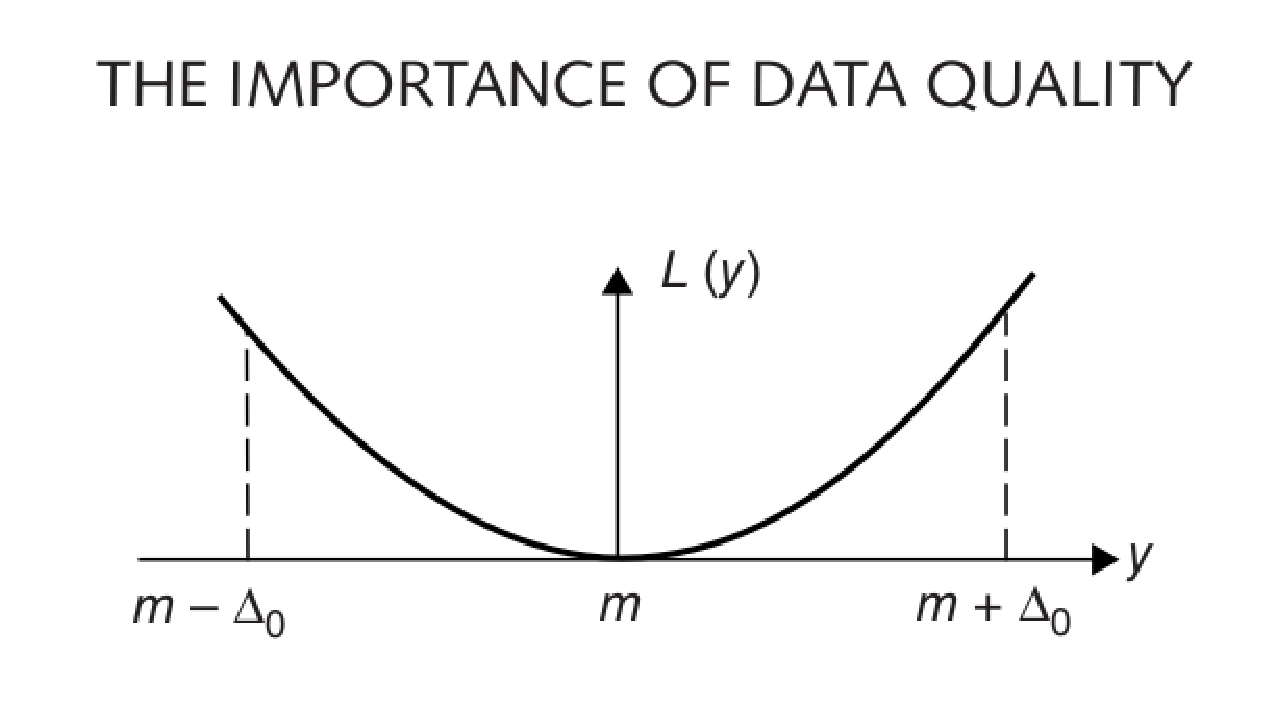
\includegraphics[width=0.6\textwidth]{quality-loss-function}
\caption{Quality Loss Function (QLF)}
\end{figure}

the loss is zero, or at the minimum. The equation for the loss function can
be expressed as follows:

\begin{equation*}
    L(y) = k(y-m)^2
\end{equation*}

where $k$ is a factor that is expressed in dollars, based on direct costs, indirect costs, 
warranty costs, reputational costs, loss due to lost customers,
and costs associated with rework and rejection. There are prescribed ways
to determine the value of $k$.
The loss function is usually not symmetrical-sometimes it is steep on
one side or on both sides. Deming ~\citep{Deming} says that the loss function need
not be exact and that it is difficult to obtain the exact function. As most
cost calculations are based on estimations or predictions, an approximate
function is sufficient-that is, close approximation is good enough.

The concept of the loss function aptly applies in the DQ context, especially when we are measuring data quality associated with various data
elements such as customer IDs, social security numbers, and account balances. Usually, the data elements are prioritized based on certain criteria,
and the quality levels for data elements are measured in terms of percent-
ages (of accuracy, completeness, etc.). The prioritized data elements are
referred to as critical data elements (CDEs).


\section{Data Quality: Wrangling and the Big Data Life Cycle}

When talking about data quality in this document, it is done referring to the degree in
which data fits to serve for its aimed purpose ~\cite{MargaretRouse}, for example, how well a medical
record allows a nurse to identify the medicine that should be given to a patient, where
“well” comprises, among general qualities, how accurate, complete, up to date, valid
and consistent ~\cite{DAMA2013} is the information so that the task can be successfully achieved.
There are several processes required to asses and improve data quality, which include data extraction, data profiling, data cleansing and data integration ~\cite{JagadishGehrkeLabrindisPapakonstantinou}, as the
major ones; altogether in “the process by which the data required by an application is
identified, extracted, cleaned and integrated, to yield a data set that is suitable for exploration and analysis” ~\cite{NormanPaton} is known as Data Wrangling. 
Figure \ref{fig:img_big_data_life_cycle} shows how each process is placed within the big data life 
cycle ~\cite{ComputingResearchAssociation} 
~\cite{JagadishGehrkeLabrindisPapakonstantinou}, where data profiling is the step in which this research contributes to.

\begin{figure}[H]
    \centering
    \includegraphics[scale=.3]{big_data_life_cycle}
    \caption{The big data life cycle}
    \label{fig:img_big_data_life_cycle}
\end{figure}


\begin{table}[H]
    \caption{Big data life cycle processes definitions I.}
    \label{table:big_data_life_cyle_processes_definition_I}
    \centering
    \begin{tabular}{p{4.0cm} p{3.1cm} p{7cm}}
    \toprule
    \textbf{Major Process} & \textbf{Process included} & \textbf{Description} \\ 
    \bottomrule
    DATA ACQUISITION & Data identification & Data has to be first generated from the
    real world, then converted to electrical signals so it can then be recorded
    in a machine. This process is called data acquisition  ~\cite{ComputingResearchAssociation}. Identifying
    data means to provide useful metadata about its provenance, intended use, recording place and motivation,
    etc. ~\cite{Dataone2016} ~\cite{Microsoft2016}. \\
    DATA EXTRACTION AND CLEANSING &  Data extraction & This is the process in which data from
    source systems is selected and transformed into a suitable type of data according to its purpose, e.g. coordinates from a set of stored satellite images ~\cite{ComputingResearchAssociation}.    
    \\
    & \\ &  Data profiling & This refers to generating convenient metadata to 
    support measurements against quality settings previously established, and to contribute towards
    “well known data”, clearing up the structure, content and/or relationships among the data. E.g. data types,data domains, timeliness, completeness, statistics, etc.~\cite{Sandra2015} ~\cite{Kimball2008}.
    \\
    & \\ & Data cleansing & Also known as cleaning or scrubbing.
    Requires solving errors found in invalid, inconsistent, incomplete or duplicated data so the quality of the data
    can be improved. To find the errors this process relies on profiling information ~\cite{Sandra2015} ~\cite{Erhard2000}.
    \\ 
    DATA INTEGRATION, AGGREGATION AND REPRESENTATION & Data integration & Integrating data involves combining data from multiple sources into one,
    meaningful and valuable set of data ~\cite{Lenzerini2002} ~\cite{Halevy2006} ~\cite{Sandra2015}.
    \\
    \bottomrule
\end{tabular}
\end{table}

\begin{table}[H]
    \caption{Big data life cycle processes definitions II.}
    \label{table:big_data_life_cyle_processes_definition_II}
    \centering
    \begin{tabular}{p{4.0cm} p{3.1cm} p{7cm}}
    \toprule
    \textbf{Major Process} & \textbf{Process included} & \textbf{Description} \\ 
    \bottomrule   
    & \\ &  Data storing & To preserve integrated data understandable, maintaining its quality, and
    adequacy to its purpose, it is also required to develop a suitable storage
    architecture design, taking into account the type of database suitableness (e.g. relational, non-relational),
    the capacities of the database management system, etc., among all the alternatives in which data could be stored. ~\cite{ComputingResearchAssociation}
    \\
    & \\ & Data visualisation & Typically one step before analysis
    techniques. This process is about applying a graphical representation to
    the data, aimed at providing ease at future usage, transformation and understanding ~\cite{Fayyad2002} ~\cite{Ware2012} ~\cite{Philip2014}.
    \\ 
    MODELING ANALYSING & Statistics \&\ machine learning & This concerns about stating facts in
    this context, from a given dataset, by interpreting data and providing a numerical picture of it, as well as using computer systems that emulate the human learning process, saving new information and outcomes,
    closely related to artificial intelligence (AI). Parallel Parallel statistics algorithms have been proposed to approach big data ~\cite{Ryszard2013}~\cite{PhilipChen2014}.
    \\
    & \\ & Data mining & This process involves techniques to
    find latent valuable information, revealing patterns, cause-effect relations, implicit facts, etc., to hold up
    data analysis ~\cite{Chandrasekar2001} ~\cite{Philip2014} .
    \\
    \bottomrule
\end{tabular}
\end{table}

\begin{table}[H]
    \caption{Big data life cycle processes definitions III.}
    \label{table:big_data_life_cyle_processes_definition_III}
    \centering
    \begin{tabular}{p{4.0cm} p{3.1cm} p{7cm}}
    \toprule
    \textbf{Major Process} & \textbf{Process included} & \textbf{Description} \\ 
    \bottomrule   
    & \\ & Data analysis & A task done by the perceptual and
    cognitive system of an analyst, although nowadays machine learning
    and AI techniques can also be used. This is the ultimate phase in the process of obtaining the value from the
    data, by finding the significance on the insights provided by, for example,
    correlations or graphical representations. ~\cite{Ware2012}
    \\
    INTERPRETATION & Understand and verify results & This is the phase in which the information obtained is used and trans-
    formed into a decision that could lead
    to a tangible value (e.g. economic gaining, marketing advantages, scientific progress ), differing each time
    according to the context on which it has been obtained and its purpose This phase also comprises retracing
    the results obtained, verifying them and testing them in several use cases
    ~\cite{ComputingResearchAssociation}.
    \\
    \bottomrule
\end{tabular}
\end{table}

In order to support the value characteristic of the data it is important to satisfy
high quality conditions of the large data sets ~\cite{ZhuCai2015}, where quality could be measured
by its dimensions, having completeness, uniqueness, timeliness, validity, accuracy and
consistency considered as the six core ones ~\cite{DAMA2013}, among other identified dimensions,
such as reputation, security, transactability, accesibility and interpretability ~\cite{Pipino2002} ~\cite{McGilvary2008}.
The processes, technologies and techniques aimed at obtaining the value from big
data, are known as big data analytics ~\cite{Kwon2014}, applied in several ambits, such as health
care, social sciences, environmental and natural resources area, business and economic
domains, and technology fields. Recently, big data quality has been approached from a
big data analytics point of view ~\cite{Kambatla2014} ~\cite{Hazen2014} ~\cite{Lavalle2011}. Some studies might conclude that data
quality is not a bigger challenge than the lack of knowledge from analysts to implement 

the correct methods to manage big data value ~\cite{Lavalle2011}, however, data management is an
inherent phase of the big data analytics, and it involves the capacity to gather, integrate
and analyse data as well, where data quality should not be considered as a separate
phase.
The Data Warehousing Institute estimated low quality data cost U.S. businesses
more than 600 billion USD per annum ~\cite{Eckerson2002}. The U.S. Postal Service estimated that
wrong data cost 1.5 billion USD in 2013 from mailpieces that could not been delivered
to the given addresses, facing data quality problems from around 158 billion mailpieces
in that single year. Data quality management strategies were recommended to increase
address information accuracy, timeliness and completeness ~\cite{USAPostService2014}. In big data, “low”
error rates translate into millions of faults annually, where the risk is to lose 10-25\%\ of
the total revenues from it ~\cite{Eckerson2002}.
Big data quality requires multidisciplinary participation to progress ~\cite{Hazen2014} and propel the development of simple and low-cost data quality techniques, reduce the cost of
poor quality data, the data error rate, and the need of data cleansing processes which
involve investing not only budget, but time and effort to manage. IS research is demanded to collaborate with data wrangling insights and advances, working together
with statistical experts to leverage the techniques involved, where domain specific authorities are needed to set the data analytics management, which should support the
right value retrieval out of relevant problems from each area ~\cite{Hazen2014}.

\section{Big Data and Parallelism}

The term big data itself comprises a deeper meaning, being not only a term to be
defined but the name of a phenomenon and an emerging discipline [34]. The earliest
mentions of big data were made, to the best of my knowledge, in 1979 by Lawrence
Stone, when describing the work of cliometricians dealing with “vast quantities of data
using electronic computers to process it and applying mathematical procedures” [121],
and by Charles Tilly, who in 1980 describing the work done by the former, used the
term “big-data people” referring to the cliometricians Stone mentioned before [138].
Then, in 1997 Michael Cox and David Ellsworth, described the term as large data
sets that surpasses the available size in main memory, local disk and even remote disk
[19]. Following that year, Sholom M. Weiss and Nitin Indurkhya in their book “Predictive data mining: a practical guide”, contextualize not only the term but the phe-
nomenon, mentioning that “millions or even hundreds of millions of individual records can lead to much stronger conclusions, making use of powerful methods to examine
data more comprehensively” and also acknowledges that analysing big data, in practice, has many difficulties [146]. Two years later, Francis X. Diebold defined big data
as “the explosion in the quantity of available and potentially relevant data, largely the
result of recent and unprecedented advancements in data recording and storage technology” [33]. By this time, it was clear that big data was not only about size, but about
the insights that a large set of data could eventually bring.

The Oxford English Dictionary, which added the term to its data base in 2013
[101], defines big data as “data of a very large size, typically to the extent that its
manipulation and management present significant logistical challenges” [102].

Nevertheless, those “logistical challenges” for one organization could be necessary
to be done when facing a smaller size of data compared to another [81], in this sense,
it seemed that relying only in the size depends on the available technology within
each organization and its capability to handle a given amount of data, so, to scope the
definition, the size of big data could be thought as the size in which using traditional
techniques to process it, is not longer an option. 

The above led to define big data not only regarding size, but taking into account
another identified characteristics, known as the “V’s of big data” [58, 82]: Volume,
Velocity, Variety, Veracity and Value; where Volume refers to the data size, Velocity
evokes the high speed of change and fast generation of data, Variety relates to the
different type of data (structured, unstructured and semistructured), Veracity is the
degree of trustworthiness of the data (quality and accuracy) and Value indicates the
worth or benefit of gathering, storing, processing and analysing the data.

Because of the nature of big data, traditional approaches to managing data are not
suitable, for example, since the main aim was to handle relational data, and as previ-
ously mentioned, big data is not always relational, so, traditional techniques are not ex-
pected to work correctly [49]. When processing data, one of the main challenges faced
with big data is the large volume of it; this require scaling, and there have been two
types of scaling for big data processing: scaling-up and scaling-out, where the former
is about implementing powerful machines, with great memory and storage capacity,
as well as quick but expensive processors, and the latter refers to the usage of several
commodity machines connected as clusters, having a parallel environment, suitable to
handle large volumes of data, and an advantageous price-performance relation, com-
pared to the scaling-up approach [88, 49]. For big data frameworks, it is known that with the proper optimisations, scaling-up performs better than scaling-out [6], how-
ever, it is still unknown exactly when is better to opt for one approach or the other,
this is, the results presented were not dependable on the framework solely, but on the
processed data characteristics. Nevertheless, it might be strongly preferred to utilise
several smaller machines than high performance computer systems (HPC), because of
the higher cost scaling-up represents, and considering the support that new paradigms
provide by avoiding the necessity to communicate data, but having the processing ap-
plications running where the data is, which proposes a significant performance advan-
tage [128], trading off performance in certain degree for a better cost-benefit ratio.

Distributed and parallel computation are two major ways of processing big data,
where a distributed system communicates and coordinates their processes without a
global clock, through messages, and in a component’s independence working as sin-
gle system [127], and parallel computing is a term generally used to identify those
processes carried out simultaneously by numerous processors, intended to reduce the
runtime [5]. Besides solely parallel, distributed or a mixture of both, new techniques
are being developed and selected towards aiding the whole big data life cycle. Recent
studies target “granular computing, cloud computing, biological computing systems
and quantum computing” [15] as the emergent areas, theories and techniques for big
data.

\section{Why Data Quality is Relevant}

The consequences of poor quality of data are often experienced in everyday life, but often, without making the necessary connections to their causes.

For example, the late or mistaken delivery of a letter is often blamed on a postal service, although  a closer look often reveals data-related causes, typically an error in the address, orginating in the address database.

Data quality has serious consequences of far-reaching significance, for the efficiency and effectiveness of organizations and business.



\section{Why Data Quality is Matters}

Poor data quality is enemy number one to the widespread, profitable use of machine learning. While the caustic observation, “garbage-in, garbage-out” has plagued analytics and decision-making for generations, it carries a special warning for machine learning. The quality demands of machine learning are steep, 
and bad data can rear its ugly head twice - first in the historical data used to train the predictive model and second in the new data used by that model to make future decisions. ~\cite{RedmanHBR2018}

Data quality is no less troublesome in implementation. Consider an organization seeking productivity gains with its machine learning program. While the data science team that developed the predictive model may have done a solid job cleaning the training data, it can still be compromised by bad data going forward. Again, it takes people — lots of them — to find and correct the errors. This in turns subverts the hoped-for productivity gains. Further, as machine learning technologies penetrate organizations, 
the output of one predictive model will feed the next, and the next, and so on, even crossing company boundaries. The risk is that a minor error at one step will cascade, causing more errors and growing ever larger across an entire process.

Bad data costs the U.S. \$3 trillion per year, IBM’s estimate of the yearly cost of poor quality data, in the US alone, in 2016. While most people who deal in data every day know that bad data is costly, this figure stuns. ~\cite{ibmInfoGraphic}


Importantly, the benefits of improving data quality go far beyond reduced costs. It is hard to imagine any sort of future in data when so much is so bad. Thus, improving data quality is a gift that keeps giving — it enables you to take out costs permanently and to more easily pursue other data strategies. 
For all but a few, there is no better opportunity in data.

\begin{figure}[H]
    \centering
    \includegraphics[angle=-90,scale=.3]{4-Vs-of-big-data}
    \caption{IBM data scientists break big data into four dimensions: volume, variety, velocity and veracity. This infographic explains and gives examples of each. ~\cite{ibmInfoGraphic}}
\end{figure}

\section{Data Quality and Types of Information Systems}

Data are collected, stored, elaborated, retrieved, and exchanged in information systems used in organizations to provide services to business processes.
Different criteria can be adopted for classifying the different types of information systems, and their corresponding architectures; they are usually related to
the overall organizational model adopted by the organization or the set of the
organizations that make use of the information system.

The three classifications are represented together in the classification space of Figure 1.2.
Among all possible combinations, five main types of information systems are highlighted in the figure:
Monolithic, Distributed, Data Warehouses,Cooperative, and Peer-to-Peer.


\begin{itemize}
    \item{In a \textit{monolithic information system} presentation, application logic, and data management are merged into a single computational node.
    Many monolithic information systems are still in use. While being extremely rigid, they provide advantages to organizations, such as reduced costs due to homogenetiy of solutions and centralization of management.
    In monolithic systems data flows have a common format, and data quality control is facilitated by the homogenetiy and centralization of procedures and management rules.}
    \item {A \textit{data warehouse} (DW) is a centralized set of data collected from different sources, designed to support management decision making. The most critical problem in DW design concerns the cleaning and integration of 
    the different data sources that are loaded into the DW, in that much of the implementation budget is spent on data cleaning activities.}
    \item{A \textit{distributed information system} relaxes the rigid centralization of monolithic systems, in that it allows the distribution of resources and applications across
    network of geographically distributed systems.
    The network can be organized in terms of several tiers, each made of one or more computational nodes. Presentation, application logic, and data management are distributed across tiers. Usually, the different tiers and nodes have a limited degree of autonomy, 
    data design is usually performed centrally, but to a certain extent some degree of heterogenetiy can occur, due to the impossibility of establishing unified procedures.
    Problems of data management are more complex than in monolithic systems, due to the reduced level of centralization.
    }  
\end{itemize}

\begin{figure}[H]
% \vspace*{.0in}
\centering
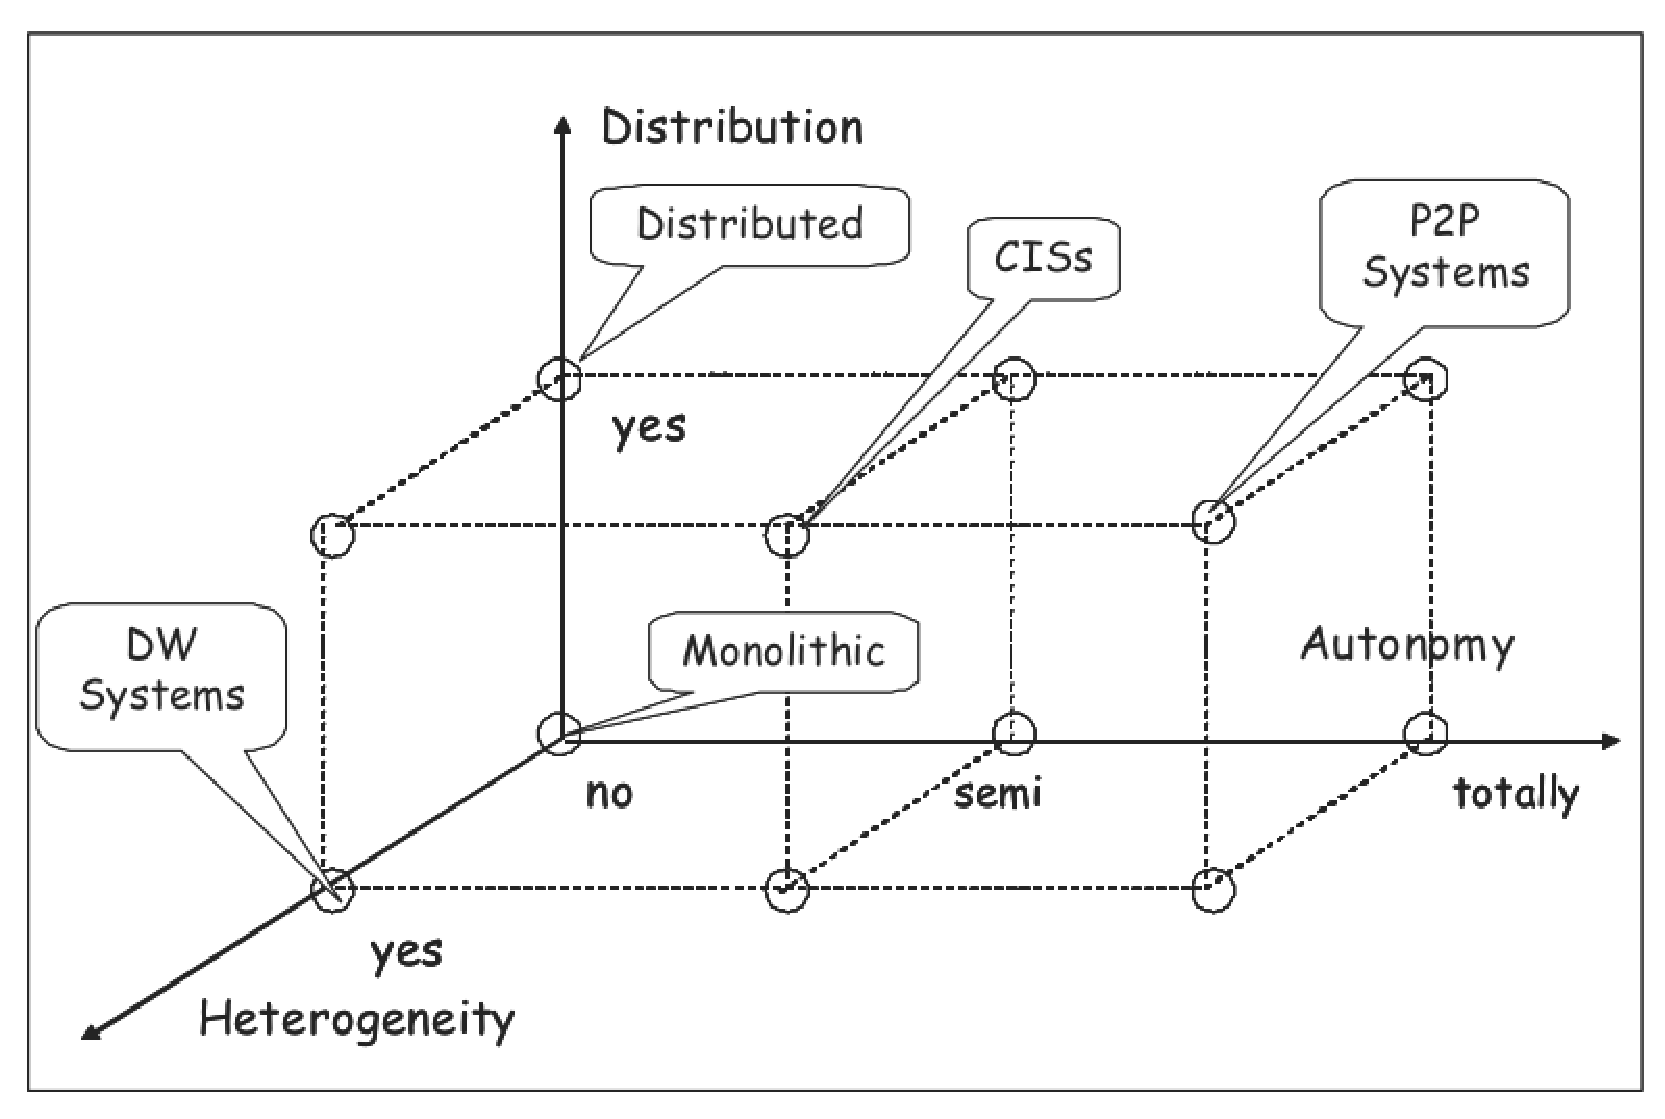
\includegraphics[scale=.50]{types-of-information-systems}
\caption{Types of information systems}    
\end{figure}

\begin{itemize}
    \item{A \textit{coorparative information system} (CIS) can be defined as a large-scale information system that interconnects various systems of different and autonomous organizations, 
    while sharing common objectives.}
    \item{In a \textit{peer to peer information system} (usually abbreviated P2P), the traditional distinction between clients and servers typical of distributed systems is disappearing.
    A P2P system can be characterized by a number of properties: peers are highly autonomous and higly heterogeneous, they have no obligation for the quality of their services
    and data, no central coordination and no central database exist, no peer has a global view of the system, global behavior emerges from local intreactions.    
    }
\end{itemize}


\section{Main Research Issues and Application Domains in Data Quality}
Due to the relevance of data quality, its nature, and the variety of data types and information systems, achieving data quality is a complex, multidisciplinary 
area of investigation. I involves several research topics and real-life application areas

\begin{figure}[H]
%\vspace*{.0in}
\centering
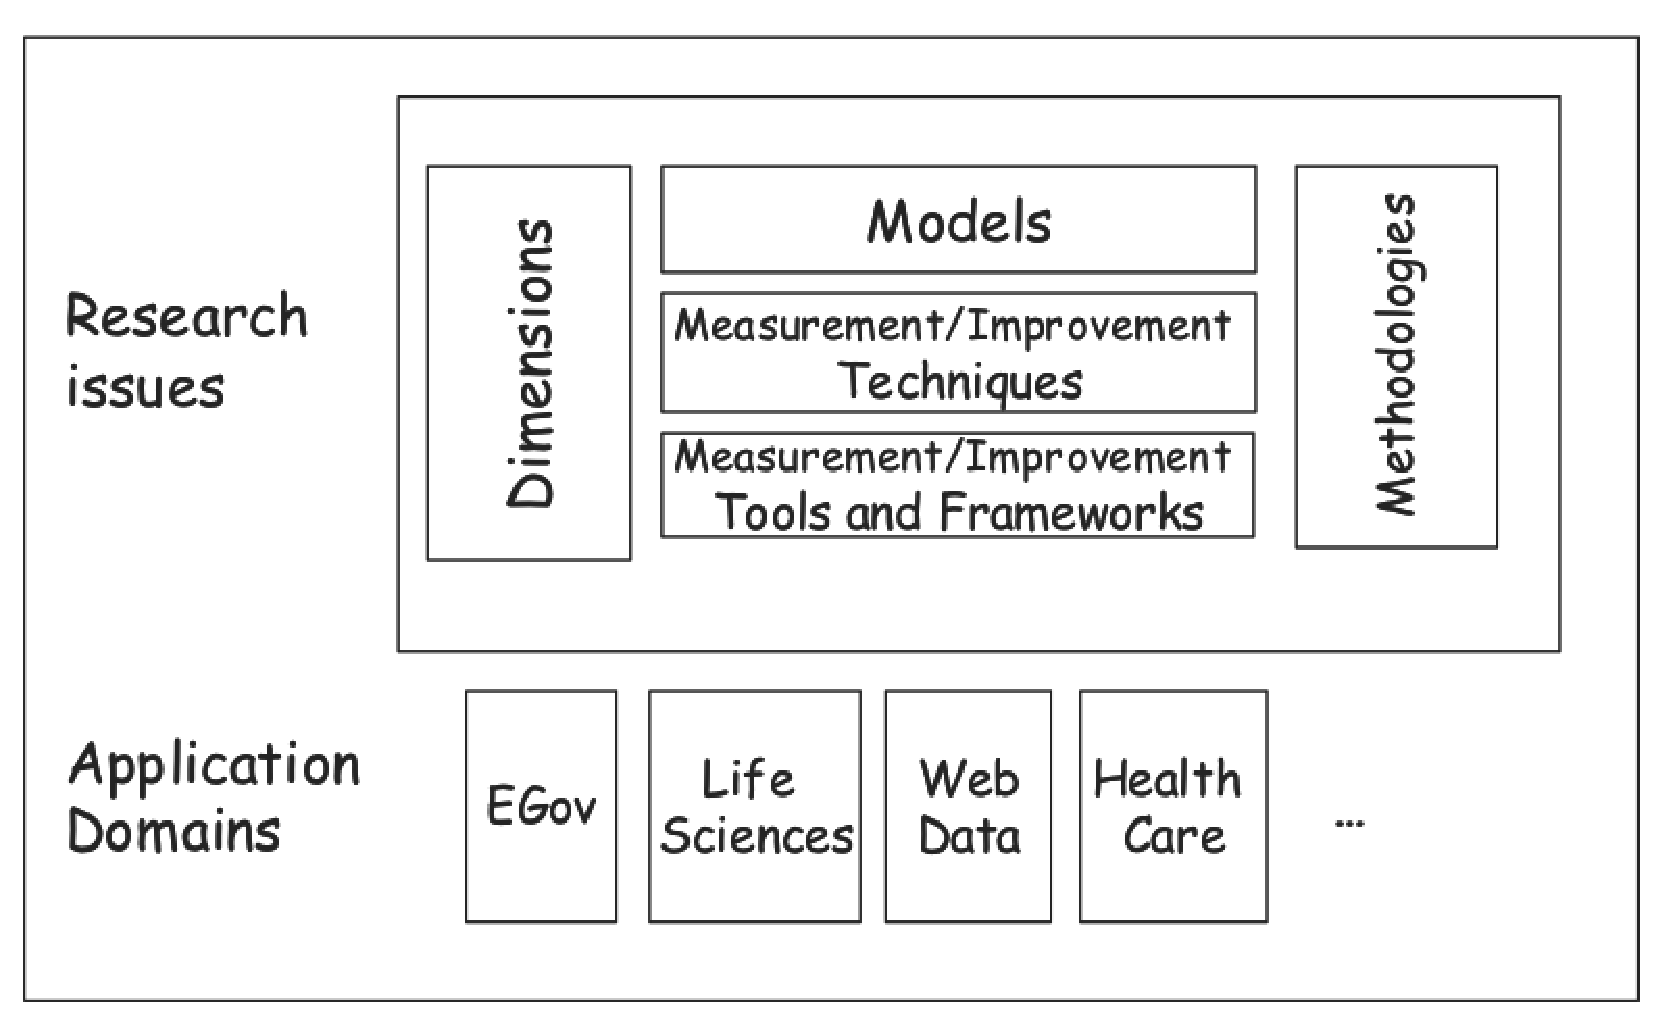
\includegraphics[scale=.50]{main-issues-in-dq}
\caption{Main issues in data quality}    
\end{figure}